%&pdflatex
\documentclass[
aps,%
12pt,%
final,%
notitlepage,%
oneside,%
onecolumn,%
nobibnotes,%
nofootinbib,%
superscriptaddress,%
noshowpacs,%
showkeys,%
centertags]%
{revtex4}

\usepackage{wrapfig}
\usepackage{mathrsfs}

\usepackage[caption=false]{subfig}

\PassOptionsToPackage{monochrome}{xcolor}
\usepackage{tikz}
\usepackage{pgfplots}

\newcommand{\Kn}{\mathrm{Kn}}
\newcommand{\Ma}{\mathrm{Ma}}
\newcommand{\Sh}{\mathrm{Sh}}
\newcommand{\dd}{\:\mathrm{d}}
\newcommand{\pder}[2][]{\frac{\partial#1}{\partial#2}}
\newcommand{\pderder}[2][]{\frac{\partial^2 #1}{\partial #2^2}}
\newcommand{\Pder}[2][]{\partial#1/\partial#2}
\newcommand{\dzeta}{\boldsymbol{\dd\zeta}}
\newcommand{\dxi}{\boldsymbol{\dd\xi}}
\newcommand{\bzeta}{\boldsymbol{\zeta}}
\newcommand{\bxi}{\boldsymbol{\xi}}
\newcommand{\bh}{\boldsymbol{h}}
\newcommand{\be}{\boldsymbol{e}}
\newcommand{\Nu}{\mathcal{N}}
\newcommand{\Mu}{\mathcal{M}}
\newcommand{\OO}[1]{O(#1)}
\newcommand{\Set}[2]{\{\,{#1}:{#2}\,\}}

\begin{document}
\selectlanguage{russian}

\title{Численный анализ медленных неизотермических течений разреженного газа на основе асимптотической теории и проекционного метода}
\author{\firstname{О.~А.}~\surname{Рогозин}}
\email{oleg.rogozin@phystech.edu}
\affiliation{Moсковский физико-технический институт}

\date{\today}

\begin{abstract}
    \begin{flushright}
    \vspace{1em}
    {\it Памяти Оскара Гаврииловича Фридлендера (1939--2015)}
    \vspace{1em}
    \end{flushright}
    Рассматриваются медленные течения разреженного газа
    под действием значительных температурных напряжений.
    Для корректного гидродинамического описания этого класса течений
    некоторые ненавье"--~стокстовские члены должны быть включены в
    уравнение импульса.
    Предлагается метод численного анализа слаборазреженного газа
    на основе уравнений Когана"--~Галкина"--~Фридлендера
    с граничными условиями, учитывающими температурный скачок.
    Метод апробирован на нескольких примерах.
    Результаты подкреплены численным решением уравнения Больцмана
    на основе проекционного метода дискретных скоростей.
\end{abstract}

\keywords{
    уравнение Больцмана,
    уравнения Когана"--~Галкина"--~Фридлендера,
    нелинейная термострессовая конвекция,
    тепловое скольжение,
    проекционный метод
}

\maketitle

%%%%%%%%%%%%%%%%%%%%%%%%%%%%%%%%%%%%%%%%%%%
\section{Введение}
%%%%%%%%%%%%%%%%%%%%%%%%%%%%%%%%%%%%%%%%%%%

%%% Slow nonisothermal flows
С 1969 по 1974 год Оск\'{а}р Гавриилович Фридлендер (1939--2015)
совместно с Владленом Сергеевичем Галкиным (род.~1932)
под руководством Михаила Наумовича Когана (1925--2011)
развили теорию \emph{медленных неизотермических}
течений газа~\cite{Kogan1970, Kogan1971, Friedlander1974, Galkin1974, Kogan1976}.
Медленность течений следует понимать как малость числа Маха (\(\Ma\ll1\)),
а неизотермичность как присутствие в газе существенного градиента температур.
Основным импульсом упомянутых работ стала попытка учесть влияние температурных напряжений
на конвекцию газа через анализ барнеттовского приближения для слаборазреженного газа.
Несмотря на то что барнеттовские члены второго порядка малости по числу Кнудсена \(\Kn\),
при \(\Ma\sim\Kn\) (число Рейнольдса порядка единицы)
они становятся сравнимыми с ньютоновскими вязкостными напряжениями.
Таким образом, уравнения Навье"--~Стокса оказываются некорректными для
описания медленных неизотермических течений.

%%% KGF equations and its derivation
В~\cite{Kogan1970} впервые была получена система уравнений гидродинамического типа,
корректно описывающая медленные неизотермические течения слаборазреженного газа.
В литературе нет единого устоявшегося их названия,
поэтому автор предлагает ввести термин \emph{уравнения Когана"--~Галкина"--~Фридлендера}
или \emph{уравнения КГФ}.
В первых работах~\cite{Kogan1970, Kogan1971} эти уравнения были получены наиболее простым способом,
на основе разложения Чепмена"--~Энскога. Такие же уравнения получаются из разложения Гильберта~\cite{Galkin1974}.
Наиболее общая формулировка нестационарных уравнений КГФ для смеси газов изложена в~\cite{Galkin2015}.

%%% Transport coefficients
Кроме коэффициентов вязкости и теплопроводности, в уравнения КГФ входят некоторые
\emph{термострессовые} транспортные коэффициенты. Для некоторых молекулярных потенциалов они
были впервые вычислены с помощью полиномов Сонина~\cite{Burnett1935, Chapman1960}.
Для модели твёрдых сфер более точные значения получены с помощью
непосредственного численного решения соответствующих интегральных уравнений~\cite{Sone1996, Sone2002, Sone2007}.

%%% Nonlinear thermal-stress flow and its simulation
Нелинейный характер температурных напряжений в уравнениях КГФ приводит к
явлению конвекции газа под их действием (\emph{нелинейная термострессовая конвекция})~\cite{Kogan1971}.
Этот тип конвекции имеет место при отсутствии внешних сил и может возникать между равномерно нагретыми телами.
Нелинейные температурные напряжения при некоторых условиях влияют также на процессы теплопередачи~\cite{Friedlander1978}.
В результате многолетнего труда под руководством О.\,Г. Фридлендера теория медленных неизотермических течений
была подтверждена экспериментально~\cite{Friedlander1997, Friedlander2003}.
В это же время, благодаря развитию вычислительной техники, появилась возможность провести численный анализ
некоторых прикладных задач с помощью гидродинамических уравнений КГФ, а также кинетических уравнений:
на основе модельных уравнений~\cite{Alexandrov2002, Aoki2006, Alexandrov2008b, Alexandrov2011, Rykov2008}
и прямого статистического моделирования (DSMC)~\cite{Alexandrov2008a, Aoki2007}.
Для малых чисел Кнудсена и особенно медленных течений, стохастические методы крайне трудоёмки с вычислительной точки зрения,
а получаемые с их помощью решения страдают от высокого уровня статистического шума.
Детерминистические методы решения уравнения Больцмана весьма перспективны в этой области,
однако связанные с ними вычислительные трудности не были преодолены полностью до настоящего времени.

%%% Continuum limit
Асимптотический анализ уравнения Больцмана для медленных неизотермических течений
показывает, что стационарное уравнение теплопроводности некорректно описывает
разреженный газ в континуальном пределе (\(\Kn\to0\))~\cite{Bobylev1995}.
Этот факт подтверждается также численным анализом~\cite{Sone1996}.
Оказывается, что инфинитезимальное поле скоростей конечным образом влияет на температурное поле.
Такое асимптотическое поведение называется \emph{эффектом призрака}~\cite{Sone2002, Sone2007}.
Некоторые математические вопросы существования и гладкости решений уравнений КГФ обсуждаются,
например, в~\cite{Tan2016}.

%%% Boundary conditions
До настоящего времени уравнения КГФ решались численно только
с граничными условиями~\emph{теплового скольжения},
при которых температура газа на границе не претерпевает скачка.
При таких условиях температурное поле не содержит поправок порядка \(\Kn\).
Логичным расширением области адекватного описания разреженного газа является
учёт температурного скачка на границе. В таком случае решение уравнений КГФ
зависит от числа Кнудсена.

%%% Second order of Kn
Тепловое скольжение и нелинейная термострессовая конвекция "--- явления первого порядка по \(\Kn\).
Некоторые линейные эффекты второго порядка, включая скольжение около равномерно нагретого тела
и влияние кривизны граничной поверхности, также хорошо изучены~\cite{Sone2002, Sone2007, Takata2015curvature}.

%%%%%%%%%%%%%%%%%%%%%%%%%%%%%%%%%%%%%%%%%%%
\section{Основные уравнения}
%%%%%%%%%%%%%%%%%%%%%%%%%%%%%%%%%%%%%%%%%%%

Прежде всего, перейдём к безразмерным переменным.
Пусть \(L\) "--- характерная длина в рассматриваемой задаче,
а \(T^{(0)}\) и \(p^{(0)}\) "--- характерные температура и давление газа.
Тогда макроскопические переменные принимают следующий вид:
температура \(TT^{(0)}\), давление \(pp^{(0)}\),
плотность \(\rho p^{(0)}/RT^{(0)}\), скорость \(v_i(2RT^{(0)})^{1/2}\).
Функция распределения молекулярных скоростей \(f(x_i,\zeta_i)(2p^{(0)})/(2RT^{(0)})^{5/2}\)
определяется в физическом пространстве \(x_iL\) и скоростном \(\zeta_i(2RT^{(0)})^{1/2}\).
Удельная газовая постоянная \(R = k_B/m\), где \(k_B\) "--- постоянная Больцмана,
\(m\) "--- молярная масса.
Число Кнудсена \(\Kn = \ell^{(0)}/L\) определяется через характерную длину свободного пробега
\begin{equation}\label{eq:ell}
    \ell^{(0)} = \frac{k_B T^{(0)}}{\sqrt2\pi d_m^2 p^{(0)}},
\end{equation}
где радиус действия межмолекулярного потенциала взаимодействия \(d_m\)
совпадает с диаметром молекул для модели твёрдых сфер.

Стационарное уравнение Больцмана в присутствии внешней силы \(F_i (2RT^{(0)})/L\) в безразмерных переменных имеет вид:
\begin{equation}\label{eq:Boltzmann}
    \zeta_i\pder[f]{x_i} + F_i\pder[f]{\zeta_i} = \frac1k J(f,f),
\end{equation}
где интеграл столкновений
\begin{equation}\label{eq:integral}
    J(f,g) = \frac12 \int(f'g'_*+g'f'_*-fg_*-gf_*)B\dd\Omega(\boldsymbol\alpha) \dzeta_*
\end{equation}
и \(k = \sqrt\pi\Kn/2\).
\(\Omega(\boldsymbol{\alpha})\) "--- телесный угол в направлении единичного вектора \(\boldsymbol\alpha\),
\(B\) "--- функционал межмолекулярного потенциала. Для модели твёрдых сфер,
\begin{equation}\label{eq:ci_kernel}
    B = \frac{|\alpha_i(\zeta_{i*}-\zeta_i)|}{4\sqrt{2\pi}}.
\end{equation}
Макроскопические переменные выражаются через моменты функции распределения:
\begin{equation}\label{eq:macro}
    \rho = \int f \dzeta, \quad
    v_i = \frac1{\rho} \int \zeta_i f \dzeta, \quad
    T = \frac{2}{3\rho}\int(\zeta_i-v_i)^2 f \dzeta, \quad
    p = \rho T.
\end{equation}

Граничные условия диффузного отражения задаются следующим образом:
\begin{equation}\label{eq:diffuse_bc}
    f\left(\zeta_i n_i > 0\right) =
        \frac{\sigma_B}{(\pi T_B)^{3/2}} \exp\left(-\frac{\zeta_i^2}{T_B}\right), \quad
    \sigma_B = -2\left(\frac{\pi}{T_B}\right)^{1/2} \int_{\zeta_i n_i < 0} \zeta_j n_j f\dzeta,
\end{equation}
где \(n_i\) "--- единичный вектор нормали к границе, направленный внутрь газа,
а \(T_B\) и \(v_{Bi}\) "--- граничные температура и скорость.
Для стационарных задач предполагается, что \(v_{Bi}n_i = 0\).

%%%%%%%%%%%%%%%%%%%%%%%%%%%%%%%%%%%%%%%%%%%
\section{Асимптотический анализ}
%%%%%%%%%%%%%%%%%%%%%%%%%%%%%%%%%%%%%%%%%%%

В этом разделе кратко излагаются основные результаты асимптотической теории
медленных неизотермических течений на основе разложения Гильберта.
Используются обозначения, принятые в~\cite{Sone1996, Sone2002, Sone2007}.
Для простоты рассматривается только молекулярная модель упругих сфер.

\subsection{Система уравнений гидродинамического типа}

Функция распределения \(f(x_i,\zeta_i)\) и макроскопические переменные \(h = \rho, v_i, T, \dots\)
могут быть разложены в ряд по \(k\):
\begin{equation}\label{eq:expansion}
    f = f_0 + f_1k + f_2k^2 + \cdots, \quad h = h_0 + h_1k + h_2k^2 + \cdots.
\end{equation}
Если предположить, что \(\Pder[f]{x_i} = \OO{f}\),
\(v_{i0} = 0\) (медленные течения), \(F_{i0} = F_{i1} = 0\) (слабое поле внешних сил)
и подставить~\eqref{eq:expansion} в уравнение Больцмана~\eqref{eq:Boltzmann},
то для получаемых интегро-дифференциальных уравнений должны выполняться
условия разрешимости в нулевом порядке:
\begin{equation}
    \pder[p_0]{x_i} = 0, \label{eq:asymptotic0_p}
\end{equation}
в первом:
\begin{gather}
    \pder{x_i}\left(\frac{u_{i1}}{T_0}\right) = 0, \label{eq:asymptotic1_u} \\
    \pder[p_1]{x_i} = 0, \label{eq:asymptotic1_p} \\
    \frac{u_{i1}}{T_0}\pder[T_0]{x_i}
        = \frac{\gamma_2}2\pder{x_i}\left(\sqrt{T_0}\pder[T_0]{x_i}\right), \label{eq:asymptotic1_T} \\
\end{gather}
и во втором:
\begin{gather}
    \pder{x_i}\left(\frac{u_{i2}}{T_0}\right)
        + \pder{x_i}\left[\left(\frac{p_1}{p_0}-\frac{T_1}{T_0}\right)\frac{u_{i1}}{T_0}\right] = 0, \label{eq:asymptotic2_u} \\
    \begin{aligned}
    \pder{x_j}\left(\frac{u_{i1}u_{j1}}{T_0}\right)
        &-\frac{\gamma_1}2\pder{x_j}\left[\sqrt{T_0}\left(
            \pder[u_{i1}]{x_j} + \pder[u_{j1}]{x_i} - \frac23\pder[u_{k1}]{x_k}\delta_{ij}
        \right)\right] \\
        &- \frac{\bar{\gamma}_7}{T_0}\pder[T_0]{x_i}\pder[T_0]{x_j}\left(\frac{u_{j1}}{\gamma_2\sqrt{T_0}} - \frac{1}4\pder[T_0]{x_j}\right)
        = -\frac12\pder[p_2^\dag]{x_i} + \frac{p_0^2 F_{i2}}{T_0},
    \end{aligned} \label{eq:asymptotic2_p} \\
    \frac{u_{i1}}{T_0}\pder[T_1]{x_i}
        + \left[\frac{u_{i2}}{T_0} + \left(\frac{p_1}{p_0}-\frac{T_1}{T_0}\right)\frac{u_{i1}}{T_0}\right]\pder[T_0]{x_i}
        = \frac{\gamma_2}2\pder{x_i}\left(\sqrt{T_0}\pder[T_1]{x_i} + \frac{T_1}{2\sqrt{T_0}}\pder[T_0]{x_i}\right). \label{eq:asymptotic2_T}
\end{gather}
Здесь обозначены \(u_{i1} = p_0v_{i1}\), \(u_{i2} = p_0v_{i2}\) и
\begin{equation}\label{eq:dag_pressure}
    p_2^\dag = p_0 p_2
        + \frac{2\gamma_3}{3}\pder{x_k}\left(T_0\pder[T_0]{x_k}\right)
        - \frac{\bar{\gamma}_7}{6}\left(\pder[T_0]{x_k}\right)^2.
\end{equation}
Уравнения~\eqref{eq:asymptotic1_u},~\eqref{eq:asymptotic1_T},~\eqref{eq:asymptotic2_p}
для \(T_0\), \(u_{i1}\) и \(p_2^\dag\) будем называть \emph{уравнениями Когана"--~Галкина"--~Фридлендера}.
Они содержат член температурных напряжений, отсутствующий в уравнениях Навье"--~Стокса.
Сравнивая его с \(p_0^2F_{i2}/T_0\), можно увидеть, что на единицу массы газа действует сила
\begin{equation}\label{eq:gamma7_force}
    k^2\frac{\bar{\gamma}_7}{p_0^2}\pder[T_0]{x_i}\pder[T_0]{x_j}\left(\frac{u_{j1}}{\gamma_2\sqrt{T_0}} - \frac{1}4\pder[T_0]{x_j}\right).
\end{equation}
Она возникает, когда изотермические поверхности не параллельны
\begin{equation}\label{eq:nonparallel}
    e_{ijk}\pder[T_0]{x_j}\pder{x_k}\left(\pder[T_0]{x_l}\right)^2 \ne 0.
\end{equation}
В~\eqref{eq:nonparallel} использован символ Леви"--~Чивиты \(e_{ijk}\).
Движение газа под действием этой силы называется \emph{нелинейной термострессовой конвекцией}.

Важно отметить, что \(p_2^\dag\) не входит в уравнение состояния,
поэтому определяется с точностью до константы.
Поскольку член \(\partial{p_2^\dag}/\partial{x_i}\) включён в систему,
как давление в уравнениях Навье"--~Стокса для несжимаемого газа,
то для решения уравнений КГФ применяются соответствующие численные методы.

Безразмерные транспортные коэффициенты для модели твёрдых сфер равны
\begin{alignat*}{2}\label{eq:gamma_coeffs}
    \gamma_1 &= 1.270042427, &\quad \gamma_2 &= 1.922284066, \\
    \gamma_3 &= 1.947906335, &\quad \bar{\gamma}_7 &= 1.758705.
\end{alignat*}
Первые два коэффициента соответствуют вязкости \(\mu\) и теплопроводности \(\lambda\) газа, т.е.
\begin{equation}\label{eq:mu_lambda}
    \mu = \gamma_1\sqrt{T_0} \frac{p^{(0)}L}{\sqrt{2RT^{(0)}}} k, \quad
    \lambda = \frac{5\gamma_2}{2}\sqrt{T_0} \frac{p^{(0)}RL}{\sqrt{2RT^{(0)}}} k.
\end{equation}
Коэффициент \(\gamma_3\) входит в выражения температурных напряжений,
которые создают неоднородное распределение давления в газе,
но не движущую силу. Поскольку \(\bar{\gamma}_7\) положителен,
нелинейная термострессовая конвекция противоположна градиенту температур.

\subsection{Граничные условия}

Граничные условия диффузного отражения имеют вид:
\begin{gather}
    T_0 = T_{B0}, \label{eq:bc_T0} \\
    T_1 = T_{B1} + d_1\frac{T_{B0}}{p_0}\pder[T_0]{x_j} n_j, \label{eq:bc_T1} \\
    \left\{
    \begin{aligned}
        & u_{j1} (\delta_{ij}-n_in_j) =
            \left(u_{Bj1} - K_1 \sqrt{T_{B0}} \pder[T_0]{x_j}\right) (\delta_{ij}-n_in_j), \\
        & u_{j1} n_j = 0.
    \end{aligned}
    \right. \label{eq:bc_u1}
\end{gather}
Здесь \(d_1\) "--- коэффициент температурного скачка, а \(K_1\) "--- коэффициент теплового скольжения.
Для модели твёрдых сфер~\cite{Ohwada1989creep, Ohwada1989jump, Takata2015}
\begin{equation}\label{eq:slip_coefficients}
    d_1 = 2.40014, \quad K_1 = -0.64642.
\end{equation}
Поскольку \(K_1<0\), направление \emph{теплового скольжения} совпадает
с направлением градиента температуры граничной поверхности.

Решение уравнений КГФ не удовлетворяет в общем случае кинетическому граничному условию~\eqref{eq:diffuse_bc}
поскольку функция распределения значительно изменяется вблизи границы вдоль нормали к ней.
Коррекция макроскопических переменных \(h = h_0 + (h_1 + h_{K1})k + \cdots\) в кнудсеновском слое
принимает следующий вид:
\begin{gather}
    T_{K1} = \frac{T_{B0}}{p_0}\left.\pder[T_0]{x_j}\right|_0 n_j
        \Theta_1\left(\frac{p_0}{T_{B0}}\eta\right), \label{eq:correction_T} \\
    \rho_{K1} = \frac1{T_{B0}}\left.\pder[T_0]{x_j}\right|_0 n_j
        \Omega_1\left(\frac{p_0}{T_{B0}}\eta\right), \label{eq:correction_rho} \\
    \left\{
    \begin{aligned}
        & u_{jK1} (\delta_{ij}-n_in_j) =
            -\frac{\sqrt{T_{B0}}}2 \left.\pder[T_{B0}]{x_j}\right|_0
            Y_1\left(\frac{p_0}{T_{B0}}\eta\right) (\delta_{ij}-n_in_j), \\
        & u_{jK1} n_j = 0,
    \end{aligned}
    \right. \label{eq:correction_u}
\end{gather}
где \(\eta = (x_i-x_{Bi})n_i/k\), \(x_{Bi}\) "--- ближайшая к \(x_i\) точка на границе,
а \(|_0\) означает значение на границе (\(\eta=0\)).
Функции \(\Theta_1(\eta)\), \(\Omega_1(\eta)\), \(Y_1(\eta)\) убывают экспоненциально от \(\eta\)
и табулированы для модели твёрдых сфер в~\cite{Ohwada1989creep, Ohwada1989jump, Sone2002, Sone2007, Takata2015}.

Разложение в ряд граничной температуры \(T_B = T_{B0} + T_{B1}k + \cdots\) может быть выполнено
произвольным образом. Обычно полагают, что \(T_{B0}=T_B\)~\cite{Sone1996, Alexandrov2002, Aoki2007},
тогда~\eqref{eq:bc_T1},~\eqref{eq:correction_T},~\eqref{eq:correction_rho} не используются.
Асимптотическое решение можно улучшить, если привнести в него граничные условия следующего порядка.
Например, если положить \(T_1=0\) на границе,
тогда из~\eqref{eq:bc_T0} и~\eqref{eq:bc_T1} следует граничное условие,
учитывающее температурный скачок,
\begin{equation}\label{eq:boundary_temp}
    T_B = T_0 \left( 1 - \frac{d_1}{p_0}\pder[T_0]{x_j}n_j k \right),
\end{equation}
при котором температура газа на границе вычисляется с точностью \(\OO{k^2}\),
однако во всей области решение будет обладать точностью \(\OO{k}\) (это видно из~\eqref{eq:asymptotic2_T}).
Следует отметить, что граничное условие~\eqref{eq:boundary_temp} подразумевает,
что получаемое вместе с ним решение уравнений КГФ зависит от \(k\),
а следовательно, больше не является решением типа Гильберта.
Другими словами, происходит смешение членов разного порядка в~\eqref{eq:expansion},
аналогичное тому, что имеет место в методе Чепмена"--~Энскога.

\subsection{Континуальный предел}

В классической гидродинамике уравнения Навье"--~Стокса (\(\bar{\gamma}_7=0\))
с неподвижными границами (\(v_{Bi}=0\)) и условиями без скольжения (\(K_1=0\))
приводят к нулевому полю \(v_{i1}=0\) и к уравнению теплопроводности
\begin{equation}\label{eq:heat_equation}
    \pder{x_i}\left(\sqrt{T_0}\pder[T_0]{x_i}\right) = 0.
\end{equation}
В общем случае корректное распределение температур в континуальном пределе (\(k\to0\))
находится из уравнений КГФ с соответствующими граничными условиями.
Оно будет совпадать с решением~\eqref{eq:heat_equation} только для узкого класса задач.

В континуальном мире (\(k=0\)) не существует величин \(u_{i1}\) и \(p^\dag_2\),
тем не менее инфинитезимальное поле скоростей \(v_i\) конечным образом влияет на \(T\).
Такое асимптотическое поведение получило название \emph{эффекта призрака} (ghost effect)~\cite{Sone2002, Sone2007}.

\subsection{Численное решение}

Для решения системы уравнений~\eqref{eq:asymptotic1_u},~\eqref{eq:asymptotic1_T},~\eqref{eq:asymptotic2_p}
применяется метод конечных объёмов на основе распространённого в гидродинамике алгоритма SIMPLE~\cite{Aoki2007}.
Используются неравномерные разностные сетки, сгущающиеся в областях сильного изменения решения.
Граничное условие~\eqref{eq:boundary_temp} приводит к постановке третьей краевой задачи,
численное решение которой требует дополнительного внимания.
При больших значениях \(n_j\Pder[T]{x_j}\) температура на границе может принимать отрицательные значения.
Чтобы избежать этого и сохранить устойчивость численной схемы достаточно ввести фактор релаксации для граничных условий.
Кроме того, такая краевая задача имеет решение на ограниченном интервале значений \(k<k_{\max}\).
Чем больше перепад температур в задаче и кривизна поверхности, тем меньше \(k_{\max}\).
Впрочем, для б\'{о}льших \(k_{\max}\) решение уравнений КГФ не в состоянии адекватно приближать
точное кинетическое решение.

%%%%%%%%%%%%%%%%%%%%%%%%%%%%%%%%%%%%%%%%%%%
\section{Метод решения уравнения Больцмана}
%%%%%%%%%%%%%%%%%%%%%%%%%%%%%%%%%%%%%%%%%%%

В настоящей работе уравнение Больцмана, записанное в безразмерной форме,
когда длина свободного пробега является характерной длиной,
\begin{equation}\label{eq:split_transport}
    \pder[f]{t} + \zeta_i\pder[f]{x_i} = J(f),
\end{equation}
решается численно с помощью симметричного расщепления второго порядка на уравнение переноса
\begin{equation}\label{eq:split_transport}
    \pder[f]{t} + \zeta_i\pder[f]{x_i} = 0,
\end{equation}
для которого используется метод конечных объёмов с явной TVD-схемой второго порядка,
и пространственно-однородное уравнение Больцмана
\begin{equation}\label{eq:split_collisions}
    \pder[f]{t} = J(f),
\end{equation}
для которого используется проекционно-интерполяционный
метод дискретных скоростей~\cite{Tcheremissine1997, Tcheremissine2006, Dodulad2015}.
Несмотря на то что проекционный метод обладает вторым порядком аппроксимации
на равномерной скоростной сетке~\cite{Anikin2012},
функция распределения нередко терпит разрывы, например, на поверхностях с диффузным граничным условием.
Поэтому для получения удовлетворительной аппроксимации в слое Кнудсена необходимо прибегать
к измельчению сетки вблизи линии разрыва.
Кроме того, для течений с большим перепадом температур скоростная сетка должна удовлетворительно аппроксимировать
распределения как холодного газа, так и горячего, что требует измельчения сетки для малых скоростей
наравне с большим её объёмом.
Для решения этих проблем необходимо обобщение проекционного метода для неравномерных скоростных сеток.
Изложенное далее обобщение основано на методике многоточечного проецирования~\citep{Dodulad2012}.

\subsection{Дискретизация скоростного пространства}

Пусть регулярная скоростная сетка \(\mathcal{V} = \Set{\zeta_\gamma}{\gamma\in\Gamma}\) построена таким образом,
что кубатура в пространстве \(\bzeta\) выражается в виде взвешенной суммы
\begin{equation}\label{eq:bzeta_cubature}
    \int F(\bzeta) \dzeta \approx \sum_{\gamma\in\Gamma} F_\gamma w_\gamma =
        \sum_{\gamma\in\Gamma} \hat{F_\gamma}, \quad
    \sum_{\gamma\in\Gamma} w_\gamma = V_\Gamma, \quad
    F_\gamma = F(\bzeta_\gamma),
\end{equation}
где \(F(\bzeta)\) "--- произвольная интегрируемая функция,
\(V_\Gamma\) "--- полный объём скоростной сетки, \(\Gamma\) "--- некоторое множество индексов.
Тогда восьмимерная кубатурная формула в пространстве \((\boldsymbol{\omega},\bzeta,\bzeta_*)\)
может быть записана как
\begin{equation}\label{eq:nu_cubature}
    \int F(\boldsymbol{\omega},\bzeta,\bzeta_*) \dd\Omega(\boldsymbol{\omega})\dzeta\dzeta_* \approx
        \frac{4\pi V_\Gamma^2}{ \sum_{\nu\in\Nu} w_{\alpha_\nu}w_{\beta_\nu} }
        \sum_{\nu\in\Nu} F(\boldsymbol{\omega}_\nu,\bzeta_{\alpha_\nu},\bzeta_{\beta_\nu}) w_{\alpha_\nu}w_{\beta_\nu},
\end{equation}
где \(F(\boldsymbol{\omega},\bzeta,\bzeta_*)\) "--- снова произвольная интегрируемая функция.
\(\alpha_\nu\in\Gamma\), \(\beta_\nu\in\Gamma\)
и \(\boldsymbol{\omega}_\nu\in S^2 = \Set{\boldsymbol{\omega}\in\mathbb{R}^3}{|\boldsymbol{\omega}| = 1}\)
получаются из некоторого восьмимерного кубатурного правила,
\(\Nu\subset\mathbb{N}\) "--- его множество индексов.
Заметим, что численное интегрирование в~\eqref{eq:nu_cubature} выполняется по
дискретному спектру \((\bzeta,\bzeta_*)\) и непрерывному спектру \(\boldsymbol{\omega}\).

Интеграл столкновений, записанный в симметризованной форме,
\begin{equation}\label{eq:symm_ci}
    J(f_\gamma) = \frac14\int \left[
        \delta(\bzeta-\bzeta_\gamma) + \delta(\bzeta_*-\bzeta_\gamma)
        - \delta(\bzeta'-\bzeta_\gamma) - \delta(\bzeta'_*-\bzeta_\gamma)\right]
        (f'f'_* - ff_*)B \dd\Omega(\boldsymbol{\omega}) \dzeta\dzeta_*,
\end{equation}
где \(\delta(\bzeta)\) "--- дельта-функция Дирака в \(\mathbb{R}^3\),
имеет следующий дискретный аналог:
\begin{equation}\label{eq:discrete_symm_ci}
    \hat{J}_\gamma(\hat{f}_\gamma) =
        \frac{\pi V_\Gamma^2}{\sum_{\nu\in\Nu} w_{\alpha_\nu}w_{\beta_\nu}}
        \sum_{\nu\in\Nu} \left(
            \delta_{\alpha_\nu\gamma} + \delta_{\beta_\nu\gamma}
            - \delta_{\alpha'_\nu\gamma} - \delta_{\beta'_\nu\gamma}
        \right)\left(
            \frac{w_{\alpha_\nu}w_{\beta_\nu}}{w_{\alpha'_\nu}w_{\beta'_\nu}}
            \hat{f}_{\alpha'_\nu}\hat{f}_{\beta'_\nu} - \hat{f}_{\alpha_\nu}\hat{f}_{\beta_\nu}
        \right)B_\nu,
\end{equation}
где \(\delta_{\varsigma\gamma}\) "--- символ Кронекера.
В общем случае \(\bzeta_{\alpha'_\nu}\) и \(\bzeta_{\beta'_\nu}\) не попадают в \(\mathcal{V}\),
поэтому величины \(\hat{f}_{\alpha'_\nu}\), \(\hat{f}_{\beta'_\nu}\), \(w_{\alpha_\nu}\), \(w_{\beta_\nu}\)
и функции \(\delta_{\alpha'_\nu\gamma}\), \(\delta_{\beta'_\nu\gamma}\) должны быть определены некоторым образом.

Для того чтобы выполнить условие~\eqref{eq:total_mass} точно, следующая аппроксимация Максвеллиана используется:
\begin{equation}\label{eq:discrete_Maxwellian}
    \hat{f}_{M\gamma} = \rho\left[\sum_{\varsigma\in\Gamma}w_\varsigma\exp
            \left(-\frac{(\bzeta_\varsigma - \boldsymbol{v})^2}{T}\right)
        \right]^{-1}
        w_\gamma\exp\left(-\frac{(\bzeta_\gamma - \boldsymbol{v})^2}{T}\right).
\end{equation}

\subsection{Проекционно-интерполяционный метод}

Если скорости после столкновения,
\(\bzeta_{\alpha'_\nu}\notin\mathcal{V}\) и \(\bzeta_{\beta'_\nu}\notin\mathcal{V}\),
заменяются ближайшими сеточными скоростями,
\(\bzeta_{\lambda_\nu}\in\mathcal{V}\) и \(\bzeta_{\mu_\nu}\in\mathcal{V}\),
дискретный интеграл столкновений~\eqref{eq:discrete_symm_ci} теряет свойство консервативности,
и дискретный Максвеллиан~\eqref{eq:discrete_Maxwellian} перестаёт быть равновесным состоянием.
Для решения этих проблем в проекционно-интерполяционном методе применяются две специальные процедуры.
Во-первых, \(\bzeta_{\alpha'_\nu}\) проецируется на множество сеточных скоростей
\(\Set{\bzeta_{\lambda_\nu+s_a}}{a\in\Lambda}\subset\mathcal{V}\) следующим образом:
\begin{equation}\label{eq:ci_projection}
    \delta_{\alpha'_\nu\gamma} = \sum_{a\in\Lambda} r_{\lambda_\nu,a}\delta_{\lambda_\nu+s_a,\gamma}.
\end{equation}
Пусть множество индексов \(\Lambda = \Set{a}{r_{\lambda_\nu,a}\neq0}\subset\mathbb{Z}\).
\emph{Проекционные веса} \(r_{\lambda_\nu,a}\) выбираются так,
чтобы обеспечить сохранение массы, импульса и кинетической энергии, т.е.
\begin{equation}\label{eq:stencil_conservation}
    \sum_{a\in\Lambda} r_{\lambda_\nu,a} = 1, \quad
    \sum_{a\in\Lambda} r_{\lambda_\nu,a} \bzeta_{\lambda_\nu+s_a} = \bzeta_{\alpha'_\nu}, \quad
    \sum_{a\in\Lambda} r_{\lambda_\nu,a} \bzeta_{\lambda_\nu+s_a}^2 = \bzeta_{\alpha'_\nu}^2.
\end{equation}
Множество правил смещения \(\mathcal{S} = \Set{s_a}{a\in\Lambda}\)
называется \emph{проекционным шаблоном}.
Во-вторых, для того чтобы выполнить
\begin{equation}\label{eq:strict_interpolation}
    J_\gamma\left(\hat{f}_{M\gamma}\right) = 0,
\end{equation}
\(\hat{f}_{\alpha'_\nu}\) интерполируется следующим образом:
\begin{equation}\label{eq:ci_interpolation}
    \frac{\hat{f}_{\alpha'_\nu}}{w_{\alpha'_\nu}} = \prod_{a\in\Lambda}
        \left(\frac{\hat{f}_{\lambda_\nu+s_a}}{w_{\lambda_\nu+s_a}} \right)^{r_{\lambda_\nu,a}}.
\end{equation}
Этот тип интерполяции требует высоких затрат с вычислительной точки зрения,
но для медленных течений, когда функция распределения близка к максвелловской,
позволяет добиться высокой точности и низкого уровня флуктуаций.
На практике операция возведения в степень может быть выполнена с точностью \(10^{-5}\),
что позволяет в несколько раз ускорить вычисления.
Между прочим,~\eqref{eq:ci_interpolation} обеспечивает также
выполнение H-теоремы Больцмана в дискретной форме~\citep{Dodulad2013}.
Для \(\bzeta_{\beta'_\nu}\) и \(\hat{f}_{\beta'_\nu}\) все формулы аналогичны.

\subsection{Решение задачи Коши}

Обратимся теперь к пространсвенно-однородному уравнению Больцмана~\eqref{eq:split_collisions}.
Пусть \(f_\gamma^n\) обозначает приближённое решение~\eqref{eq:split_collisions}
для скорости \(\bzeta_\gamma\), \(\gamma\in\Gamma\) в момент времени \(t_n\), \(n\in\mathbb{N}\).
Переписывая~\eqref{eq:discrete_symm_ci} как
\begin{equation}\label{eq:discrete_short_ci}
    \hat{J}_\gamma^n\left(\hat{f}_\gamma^n\right) =
        \sum_{\nu=1}^N \hat{\mathscr{J}}_\gamma^{n+(\nu-1)/N} \left(\hat{f}_\gamma^n\right), \quad
    N=|\Nu|,
\end{equation}
где \(\hat{\mathscr{J}}_\gamma^{n+(\nu-1)/N}\) "--- это \(\nu\in\Nu_n\) член суммы~\eqref{eq:discrete_symm_ci},
можно применить явный метод Эйлера первого порядка в дробных шагах
\begin{equation}\label{eq:time_scheme}
    \hat{f}_\gamma^{n+\nu/N} = \hat{f}_\gamma^{n+(\nu-1)/N} + \tau \hat{\mathscr{J}}_\gamma^{n+(\nu-1)/N}
    \left(\hat{f}_\gamma^{n+(\nu-1)/N}\right),
\end{equation}
где \(\tau = t_{n+1} - t_n\) "--- временн\'{о}й шаг.
Схема~\eqref{eq:time_scheme} имеет порядок сходимости \(\OO{\tau|\Gamma|/|\Nu|}\),
если все дискретные скорости \(\bzeta_\gamma\) распределены равномерно
в последовательностях \((\alpha_\nu)_{\nu=1}^N\) и \((\beta_\nu)_{\nu=1}^N\).
Этого можно добиться случайной перестановкой кубатурной последовательности.
Если \(|\Gamma|/|\Nu| = \OO{\tau}\), второй порядок точности достигается.

%%% On the cubature rule
Решётчатое правило Коробова~\citep{Korobov1959, Sloan1994} используется в качестве
восьмимерной кубатурной формулы в~\eqref{eq:discrete_symm_ci}.
На каждом временн\'{о}м шаге решётка сдвигается на случайный вектор,
так что получается последовательность множеств кубатурных точек \((\Nu_n)_{n\in\mathbb{N}}\)

\subsection{Сохранение положительности}

Схема~\eqref{eq:time_scheme} допускает отрицательные значения функции распределения,
что противоречит её физической природе.
Для того чтобы обеспечить её положительность, достаточно потребовать
\begin{equation}\label{eq:positive_f}
    \hat{f}_\gamma^{n+(j-1)/N} + \frac{\tau}N \hat{\mathscr{J}}_\gamma^{n+(j-1)/N} > 0
\end{equation}
для всех \(\gamma\in\Gamma\) и \(\nu\in\Nu_n\).
Если \(\gamma = \alpha_\nu\), то имеем
\begin{equation}\label{eq:positive_f_alpha}
    \hat{f}_{\alpha_\nu} - \frac{A}{N}\hat{f}_{\alpha_\nu}\hat{f}_{\beta_\nu} > 0, \quad
    A = \frac{\pi\tau V_\Gamma^2 N B_{\max}}{\sum_{\nu\in\Nu} w_{\alpha_\nu}w_{\beta_\nu}}
\end{equation}
или
\begin{equation}\label{eq:positive_f_alpha2}
    N > A \hat{f}_{\max},
\end{equation}
где
\begin{equation}\label{eq:f_B_max}
    \hat{f}_{\max} = \max_{\gamma\in\Gamma} \hat{f}_\gamma, \quad
    B_{\max} = \max_{\substack{\gamma,\varsigma\in\Gamma\\\boldsymbol{\omega}\in S^2}}
        B(\boldsymbol{\omega}, \bzeta_{\gamma}, \bzeta_{\varsigma}) = \OO{\zeta_{\max}}, \quad
    \zeta_{\max} = \max_{\gamma\in\Gamma}|\bzeta_\gamma|.
\end{equation}
Такая же оценка справедлива для \(\gamma = \beta_\nu\).

Проективные узлы \(\gamma = \lambda_\nu+s_a\) (и \(\gamma = \mu_\nu+s_a\))
рассматриваются с интерполяцией~\eqref{eq:ci_interpolation}.
Дополнительно подразумеваем, что \(r_{\lambda_\nu,a} \leq 1\).
Если \(r_{\lambda_\nu,a} \geq 0\), получаем
\begin{equation}\label{eq:positive_f_lambda2+}
    N > A \hat{f}_{\max} \epsilon_f^2 \epsilon_w^2,
\end{equation}
где
\begin{equation}\label{eq:epsilon_f}
    \epsilon_f = \max_{\substack{s_a,s_b\in\mathcal{S}\\\gamma\in\Gamma}} \frac{\hat{f}_{\gamma+s_a}}{\hat{f}_{\gamma+s_b}}, \quad
    \epsilon_w = \max_{\gamma,\varsigma\in\Gamma} \frac{w_\gamma}{w_\varsigma}.
\end{equation}
Для гладкой функции распределения \(\epsilon_f\) пропорциональна максимальному \emph{диаметру} проекционного шаблона
\begin{equation}\label{eq:stencil_diameter}
    R_\mathcal{S} = \max_{\substack{s_a,s_b\in\mathcal{S}\\\gamma\in\Gamma}}
        \left| \bzeta_{\gamma+s_a} - \bzeta_{\gamma+s_b} \right|.
\end{equation}
Если \(r_{\lambda_\nu,a} < 0\), имеем
\begin{equation}\label{eq:positive_f_lambda-}
    \hat{f}_{\lambda_\nu+s_a} + \frac{A}{N}r_{\lambda_\nu,a} \hat{f}_{\alpha_\nu}\hat{f}_{\beta_\nu} > 0.
\end{equation}
Для произвольной функции распределения, получаем дорогостоящую оценку
\begin{equation}\label{eq:positive_f_lambda2-}
    N > A \hat{f}_{\max} \bar{r}_{\max} \max_{\gamma,\varsigma\in\Gamma}\frac{\hat{f_\gamma}}{\hat{f_\varsigma}}, \quad
    \bar{r}_{\max} = \max_{\gamma\in\Gamma,a\in\Lambda}( -r_{\gamma,a} ),
\end{equation}
но для Максвеллиана
\begin{equation}\label{eq:positive_f_lambda2-maxw}
    N > A \hat{f}_{\max} \epsilon_f^2 \bar{r}_{\max}.
\end{equation}

Таким образом, чтобы уменьшить количество точек \(N\), достаточное для~\eqref{eq:positive_f},
скоростную сетку необходимо строить, минимизируя \(|\Gamma|\), \(\zeta_{\max}\) и \(\epsilon_w\),
а проекционный шаблон выбирать, минимизируя \(R_\mathcal{S}\) и \(\bar{r}_{\max}\).
Величина \(\epsilon_f\) уменьшается при сгущении сетки в областях больших градиентов функции распределения.

%%% Excluding of the points
На практике условие~\eqref{eq:positive_f} для всех \(\nu\) требует больших вычислительных затрат.
Для достижения приемлемой точности, достаточно исключать из~\eqref{eq:time_scheme} члены,
нарушающие~\eqref{eq:positive_f}. Другими словами, столкновительный интеграл можно вычислять как
\begin{equation}\label{eq:discrete_short_ci_discarded}
    \hat{J}_\gamma^n = \sum_{\nu\in\Nu\setminus\Mu} \hat{\mathscr{J}}_\gamma^{n+(\nu-1)/N},
\end{equation}
где \(\Mu\) "--- множество кубатурных точек, исключённых из \(\Nu\).
Для того чтобы не допустить значительной ошибки при такой методике численного интегрирования,
необходимо контролировать вклад исключённых узлов в столкновительный интеграл.
Например, \(N\) может быть выбрано так, что следующая сумма достаточно мала:
\begin{equation}\label{eq:excluded_contribution}
    \epsilon_J = \frac{\pi V_\Gamma^2}{\rho\sum_{\nu\in\Nu} w_{\alpha_\nu}w_{\beta_\nu}}
        \sum_{\nu\in\Mu} \left|
            \hat{f}_{\lambda_\nu}\hat{f}_{\mu_\nu} - \hat{f}_{\alpha_\nu}\hat{f}_{\beta_\nu}
        \right|B_\nu.
\end{equation}
Интерполяция~\eqref{eq:ci_interpolation} может приводить к огромным значениям \(\hat{f}_{\alpha'_\nu}\),
когда одно из значений \(\hat{f}_{\lambda_\nu+s_a}\) очень мало,
а соответствующий ему вес \(r_{\lambda_\nu,a}\) отрицателен.
По этой причине, мы избегаем интерполяции в~\eqref{eq:excluded_contribution}.

\subsection{Проекционные шаблоны}

%%% Rectangular grid
В дальнейшем будем предполагать, что скоростная сетка прямоугольна в~\(\mathbb{R}^3\),
поэтому она может быть проиндексирована целочисленным вектором, т.\,е. \(\Gamma = \Set{\gamma}{\gamma\in\mathbb{Z}^3}\).
Правило смещений может быть также представлено как целочисленный вектор, т.\,е. \(\mathcal{S}\subset\mathbb{Z}^3\).
Тогда сумму индексов следует интерпретировать как векторную сумму в~\(\mathbb{Z}^3\).

%%% Review of schemes
Благодаря симметрии равномерной сетки,
достаточно использовать два проекционных узла чтобы обеспечить консервативность.
В общем случае, пять проекционных узлов необходимо, чтобы удовлетворить~\eqref{eq:stencil_conservation}.
Диаметр шаблона \(R_\mathcal{S}\) можно уменьшить, если семь проекционных узлов использовать.
Если \(|\mathcal{S}|=n\), то схема~\eqref{eq:time_scheme} называется \(n\)-\emph{точечной схемой}.

%%% 2-point scheme
\emph{2-точечная схема} основана на симметричном проецировании
\begin{equation}\label{eq:uniform_projection}
    \delta_{\alpha'\gamma} = (1-r)\delta_{\lambda\gamma} + r\delta_{\lambda+s,\gamma}, \quad
    \delta_{\beta'\gamma} = (1-r)\delta_{\mu\gamma} + r\delta_{\mu-s,\gamma},
\end{equation}
где \(\bzeta_{\lambda+s} + \bzeta_{\mu-s} = \bzeta_{\lambda} + \bzeta_{\mu}\) и
\begin{equation}\label{eq:stencil_weights2}
    r = \frac{E_0-E_1}{E_2-E_1}, \quad
    E_0 = \bzeta_{\alpha'}^2 + \bzeta_{\beta'}^2, \quad
    E_1 = \bzeta_{\lambda}^2 + \bzeta_{\mu}^2, \quad
    E_2 = \bzeta_{\lambda+s}^2 + \bzeta_{\mu-s}^2.
\end{equation}
Подстрочный индекс \(\nu\) опущен для краткости.
Для этой схемы выполняются следующие соотношения:
\begin{equation}\label{eq:weights_ranges2}
    0 \leq r < 1, \quad h \leq R_{\mathcal{S}} \leq \sqrt3h,
\end{equation}
где \(h^3 = w_\gamma = V_\Gamma/|\Gamma|\).

%%% 5-point scheme
Пусть \(\boldsymbol{\eta} = \bzeta_{\alpha'} - \bzeta_{\lambda}\),
а \(\bh_+\), \(\bh_-\) "--- минимальные диагональные смещения от \(\bzeta_{\lambda}\),
такие что вектор \(\bh_+\) направлен в тот же октант, что и \(\boldsymbol{\eta}\),
а вектор \(\bh_-\) лежит в противоположном.
Тогда \emph{компактная 5-точечная схема} строится на узлах
\begin{equation}\label{eq:stencil_nodes5}
    \bzeta_{\lambda+s_0} = \bzeta_{\lambda}, \quad
    \bzeta_{\lambda+s_i} = \bzeta_{\lambda} + (\bh_+\cdot \be_i)\be_i, \quad
    \bzeta_{\lambda+s_4} = \bzeta_{\lambda} + \bh_-,
\end{equation}
где \(\be_i\) "--- базис прямоугольной скоростной сетки.
Проекционные веса, удовлетворяющие~\eqref{eq:stencil_conservation}, равны
\begin{equation}\label{eq:stencil_weights5}
    r_{\lambda,0} = 1 - \sum_{j=1}^4 r_{\lambda,j}, \quad
    r_{\lambda,i} = \frac{\eta_i - r_{\lambda,4}h_{-i}}{h_{+i}}, \quad
    r_{\lambda,4} = \frac{\boldsymbol{\eta}\cdot(\boldsymbol{\eta} - \bh_+)}
        {\bh_-\cdot(\bh_- - \bh_+)}.
\end{equation}
Для равномерной сетки справедливы следующие соотношения:
\begin{equation}\label{eq:weights_ranges5}
    0 < r_{\lambda,0} \leq 1, \quad
    -\frac1{12} \leq r_{\lambda,i} < \frac{11}{24}, \quad
    -\frac18 \leq r_{\lambda,4} \leq 0, \quad
    R_\mathcal{S} = \sqrt6h.
\end{equation}

%%% 7-point scheme
\emph{Симметричная 7-точечная схема} строится на узлах
\begin{equation}\label{eq:stencil_nodes7}
    \bzeta_{\lambda+s_0} = \bzeta_{\lambda}, \quad
    \bzeta_{\lambda+s_{\pm i}} = \bzeta_{\lambda} + (\bh_\pm\cdot \be_i)\be_i.
\end{equation}
Проекционные веса, удовлетворяющие~\eqref{eq:stencil_conservation}, равны
\begin{equation}\label{eq:stencil_weights7}
    r_{\lambda,0} = 1 - \sum_{j=1}^3 r_{\lambda,j} + r_{\lambda,-j}, \quad
    r_{\lambda,\pm i} = \pm\frac{\eta_i(\eta_i - h_{\mp i})}{h_{\pm i}(h_{+i}-h_{-i})}.
\end{equation}
В~\eqref{eq:stencil_weights7} суммирование по повторяющимся индексам не производится.
Для равномерной сетки справедливы следующие соотношения:
\begin{equation}\label{eq:weights_ranges7}
    \frac14 \leq r_{\lambda,0} \leq 1, \quad
    0 \leq r_{\lambda,\pm i} \leq \frac38, \quad
    -\frac18 \leq r_{\lambda,\mp i} \leq 0, \quad
    R_\mathcal{S} = 2h.
\end{equation}

И 5-точечная, и 7-точечная схемы обладают \(\bar{r}_{\max}=1/8\).
Для того чтобы уменьшить это значение, ещё больше проекционных узлов необходимо использовать~\citep{Dodulad2012}.

%%%%%%%%%%%%%%%%%%%%%%%%%%%%%%%%%%%%%%%%%%%
\section{Численные примеры}
%%%%%%%%%%%%%%%%%%%%%%%%%%%%%%%%%%%%%%%%%%%

%%% SNIT solver
В настоящей работе уравнения КГФ~\eqref{eq:asymptotic1_u},~\eqref{eq:asymptotic1_T},~\eqref{eq:asymptotic2_p}
решаются с помощью солвера \verb+snitSimpleFoam+~\cite{Rogozin2014},
использующего метод конечных объёмов на основе вычислительной платформы OpenFOAM\textregistered{}.
Сетки подбираются таким образом, чтобы обеспечить численную ошибку не более \(10^{-4}\).
Итерационный процесс обрывается, когда невязка становится меньше \(10^{-5}\).

%%% Boltzmann solver
Программная реализация описанного алгоритма численного решения уравнения Больцмана
осуществлена в рамках проблемно-моделирующей среды
для анализа газокинетических процессов~\cite{Kloss2011, Kloss2012}.
Сетки в физическом пространстве выбираются по такому же критерию, как и для численного решения уравнений КГФ,
однако дополнительно сгущаются в геометрической прогрессии возле границ с диффузным отражением,
чтобы обеспечить аппроксимацию слоя Кнудсена с ошибкой не более \(10^{-4}\).
Сетки в скоростном пространстве выбираются как равномерные, так и неравномерные,
причём начальная функция распределения при моделировании на подробной сетке всегда бралась
как результат моделирования на грубой сетке.
Для неравномерных сеток используется компактная 5-точечная схема, поскольку она требует
немного меньших вычислительных затрат по сравнению с 7-точечной.
Множество кубатурных точек обеспечивает \(\epsilon_J < 10^{-4}\).

\subsection{Задача Соне"--~Бобылева}

\begin{wrapfigure}{r}{7.4cm}
    \vspace{-10pt}
    \centering
    \includegraphics{Fig01}
    \vspace{-20pt}
    \caption{Геометрия задачи Соне"--~Бобылева}\label{fig:sone_bobylev}
    \vspace{20pt}
\end{wrapfigure}

Рассмотрим плоскую периодическую геометрию, как на рис.~\ref{fig:sone_bobylev}.
Газ расположен между двумя покоящимися (\(v_{Bi} = 0\)) бесконечными параллельными пластинами,
разделёнными на единичное расстояние. Их температура распределена по синусоидальному закону:
\begin{equation}
    T_B = 1 - \frac{\cos(2\pi x)}{2}.
\end{equation}
В качестве граничного условия на пластинах используется полное диффузное отражение.
Плотность газа нормирована на единицу, т.е.
\begin{equation}\label{eq:total_mass}
    \int_0^1\int_0^1\rho\dd{x}\dd{y} = 1.
\end{equation}

В силу симметрии задачи, расчётная область представляет собой квадрат со стороной \(1/2\).
На рис.~\ref{fig:sone_bobylev} выделена серым цветом.
Подобная задача изучалась в~\cite{Sone1996} как с помощью уравнений КГФ, так и на основе кинетического подхода,
однако из-за высокой сложности численного решения уравнения Больцмана, использовалось модельное уравнение.
Некоторые результаты моделирования смеси газов для рассматриваемой геометрии можно найти в~\cite{Wu2015}.
В настоящей работе получено прямое решение уравнения Больцмана для модели твёрдых сфер.
Кроме того, в рамках задачи рассмотривается приближённое решение гидродинамического типа для малых \(\Kn\),
основанное на граничном условии с учётом температурного скачка~\eqref{eq:boundary_temp}.

\subsubsection{Решение задачи в континуальном пределе}

\begin{figure}
    %\centering
    \subfloat[уравнение теплопроводности~\eqref{eq:heat_equation}]{
        \includegraphics[width=0.5\textwidth]{Fig02}
        \label{fig:continuum:temp-heat}
    }
    \subfloat[уравнения КГФ]{
        \includegraphics[width=0.5\textwidth]{Fig03}
        \label{fig:continuum:temp-snit}
    }
    \caption{Изотермические линии в континуальном пределе}
    \label{fig:continuum:temp}
\end{figure}

\begin{figure}
    \centering
    \subfloat[уравнения КГФ без скольжения (\(K_1=0\))]{
        \includegraphics[width=0.5\textwidth]{Fig04}
        \label{fig:continuum:flow-nonslip}
    }
    \subfloat[уравнения КГФ]{
        \includegraphics[width=0.5\textwidth]{Fig05}
        \label{fig:continuum:flow-snit}
    }
    \caption{Стационарное поле \(v_{i1}\) в континуальном пределе:
        изолинии соответствуют модулю, кривые со стрелками изображают направление}
    \label{fig:continuum:flow}
\end{figure}

%%% Space discretization
Для численного решения поставленной задачи в физическом пространстве
используется следующая прямоугольная сетка:
область \(0<x<1/2\) разбивается на 30 интервалов одинаковой длины,
а область \(0<y<1/2\) на 40 интервалов, сгущающихся к \(y=0\).

%%% Results and discussions
На рис.~\ref{fig:continuum:temp} показано стационарное температурное поле,
получаемое как при решении уравнения теплопроводности, так и уравнений КГФ.
В континуальном пределе уравнение теплопроводности получается из уравнений КГФ,
если положить \(\bar{\gamma}_7=0\) и \(K_1=0\).
Эффект теплового скольжения газа значительно превышает влияние нелинейной термострессовой конвекции,
что продемонстрированно на рис.~\ref{fig:continuum:flow}, где уравнения КГФ решены
для граничных условий со скольжением и без.
Отметим также, что направления течения газа противоположны на рис.~\ref{fig:continuum:flow-nonslip}
и~\ref{fig:continuum:flow-snit}.
Полученные результаты в континуальном пределе совпадают с представленными в~\cite{Sone1996}.
Этот факт может служить верификацией используемого солвера \verb+snitSimpleFoam+.

\subsubsection{Решение для произвольных чисел Кнудсена}

\begin{figure}
    \centering
    \subfloat[уравнения КГФ с граничным условием~\eqref{eq:boundary_temp}]{
        \includegraphics[width=0.5\textwidth]{Fig06}
        \label{fig:kn0.01:temp-snit}
    }
    \subfloat[уравнение Больцмана]{
        \includegraphics[width=0.5\textwidth]{Fig07}
        \label{fig:kn0.01:temp-exact}
    }
    \caption{Изотермические линии для \(\Kn=0.01\)}
    \label{fig:kn0.01:temp}
\end{figure}

\begin{figure}
    \centering
    \subfloat[уравнения КГФ с граничным условием~\eqref{eq:boundary_temp}]{
        \includegraphics[width=0.5\textwidth]{Fig08}
        \label{fig:kn0.01:flow-snit}
    }
    \subfloat[уравнение Больцмана]{
        \includegraphics[width=0.5\textwidth]{Fig09}
        \label{fig:kn0.01:flow-exact}
    }
    \caption{Стационарное поле скоростей для \(\Kn=0.01\):
        изолинии соответствуют модулю, кривые со стрелками изображают направление}
    \label{fig:kn0.01:flow}
\end{figure}

\begin{figure}
    \centering
    \subfloat[изотермические линии]{
        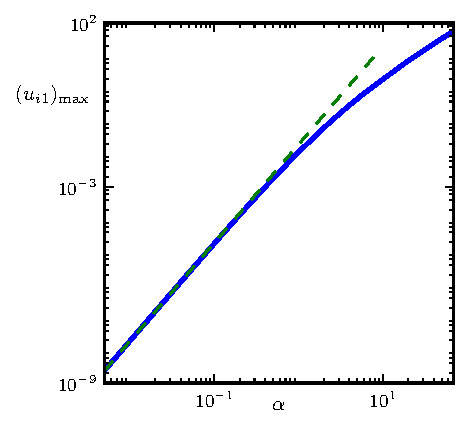
\includegraphics[width=0.5\textwidth]{Fig10}
        \label{fig:kn0.1:temp}
    }
    \subfloat[поле скоростей]{
        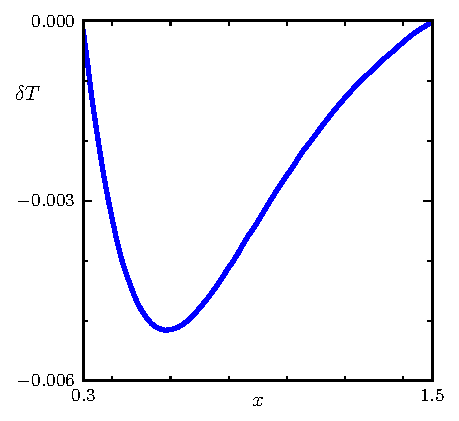
\includegraphics[width=0.5\textwidth]{Fig11}
        \label{fig:kn0.1:flow}
    }
    \caption{Решение уравнения Больцмана для \(\Kn=0.1\)}
    \label{fig:kn0.1}
\end{figure}

%%% Space discretization
Для рассмотрения задачи в произвольном диапазоне чисел Кнудсена необходимо
обратиться к численному решению уравнения Больцмана.
В физическом пространстве использовалась такая же разностная сетка,
как и при решении уравнений гидродинамического типа,
однако в слое Кнудсена (вблизи \(y=0\)) она дополнительно сгущалась так,
что ширина приграничной ячейки равнялась \(0.02\) от длины свободного пробега.
Для контроля точности использовались две различные сетки в скоростном пространстве.
Сначала задача решалась на равномерной прямоугольной сетке, ограниченной сферой радиусом \(4.24\),
так что на радиусе помещалось 8 ячеек.
Далее результат уточнялся на неравномерной сетке, ограниченной сферой радиусом \(5.3\),
причём вдоль осей \(x\) и \(z\) границы ячеек располагались как корни полинома Эрмита,
а вдоль оси \(y\) сгущались в геометрической прогрессии так,
что ширина ячеек возле \(y=0\) равнялась \(0.0067\).
Таким образом, на радиусе помещалось 9, 26, 9 ячеек соответственно.
Множества кубатурных точек также имели разную мощность: около \(5\cdot10^3\) для равномерной сетки
и около \(2\cdot10^5\) для неравномерной.
Кроме того, для очень малых \(\Kn\) применялась временн\'{а}я экстраполяция распределения температуры
и поля скоростей, поскольку достижение стационарного состояния вблизи \(y=1/2\)
требует слишком большого числа итераций.

%%% Results and discussions
На рис.~\ref{fig:kn0.01:temp} и~\ref{fig:kn0.01:flow} изображено поле температуры и скорости
для \(\Kn=0.01\) и проводится сравнение между численным решением уравнения Больцмана
и приближённым решением для малых \(\Kn\).
На рис.~\ref{fig:kn0.1} показаны соответствующие распределения для \(\Kn=0.1\).
С увеличением \(\Kn\) возрастает поток теплового скольжения и температурный скачок возле границы \(y=0\).
При этом область максимальной скорости газа отодвигается от пластины.

\newcommand*{\graphlinewidth}{1}
\pgfplotscreateplotcyclelist{legend}{
    {cyan,  dashdotted, line width=\graphlinewidth},
    {blue,  solid,      line width=\graphlinewidth},
    {green, dashed,     line width=\graphlinewidth},
    {red,   dashed,     line width=\graphlinewidth, mark=o, mark options={solid}},
    {magenta, dotted,     line width=\graphlinewidth, mark=square, mark options={solid}},
}
\newcommand{\pgfplotsReferenceGenerator}[3]{
    \scalebox{0}{
        \begin{tikzpicture}
            \begin{axis}[hide axis, cycle list name = #1]
                \foreach \i   [evaluate=\i] in {1,...,#2}{
                    \addplot (0,0); \label{#3\i}
                }
            \end{axis}
        \end{tikzpicture}
    }
}

\pgfplotsReferenceGenerator{legend}{5}{line}

\begin{figure}
    \centering
    \subfloat[]{
        \includegraphics[width=0.5\textwidth]{Fig12}
        \label{fig:comparison:bottomT}
    }
    \subfloat[]{
        \includegraphics[width=0.5\textwidth]{Fig13}
        \label{fig:comparison:bottomU}
    }\\
    \subfloat[]{
        \includegraphics[width=0.5\textwidth]{Fig14}
        \label{fig:comparison:topT}
    }
    \subfloat[]{
        \includegraphics[width=0.5\textwidth]{Fig15}
        \label{fig:comparison:topU}
    }
    \caption{
        Некоторые пограничные интегралы в зависимости от \(\Kn\), полученные разными методами:
        уравнение теплопроводности~\ref{line1},
        уравнения КГФ с условием~\eqref{eq:boundary_temp}~\ref{line2} и без~\ref{line3},
        уравнение Больцмана на равномерной~\ref{line4} и неравномерной~\ref{line5} сетках
    }
    \label{fig:comparison}
\end{figure}

%%% Comparison between solutions
Чтобы наглядно продемонстрировать сходимость численного решения уравнения Больцмана к
решению уравнений КГФ в континуальном пределе, рассмотрим рис.~\ref{fig:comparison}.
На рис.~\ref{fig:comparison:topT} отчётливо видно, что решение уравнения Больцмана сходится
именно к решению уравнений КГФ, а не уравнения теплопроводности.
Для самых малых \(\Kn\) погрешность решения уравнения Больцмана возрастает
ввиду получения стационарного значения посредством экстраполяции.
На рис.~\ref{fig:comparison:bottomT} приближённое решение гидродинамического типа
на основе граничного условия~\eqref{eq:boundary_temp} аппроксимирует
точное решение со вторым порядком точности,
в то время как другие решения дают только первый порядок.
Приближённое решение отличается от точного менее чем на 10\% в области \(\Kn<0.05\),
однако стоит учитывать, что в рассматриваемой задаче тепловое скольжение значительно
превалирует над нелинейной термострессовой конвекцией.
Для противоположного случая приближённое решение может давать б\'{о}льшую погрешность.

%%%%%%%%%%%%%%%%%%%%%%%%%%%%%%%%%%%%%%%%%%%
\subsection{Течение газа между двумя эллиптическими цилиндрами}
%%%%%%%%%%%%%%%%%%%%%%%%%%%%%%%%%%%%%%%%%%%

\begin{wrapfigure}{r}{7.4cm}
    \vspace{-10pt}
    \centering
    \includegraphics{Fig16}
    \vspace{-20pt}
    \caption{Геометрия задачи}\label{fig:elliptic}
    \vspace{20pt}
\end{wrapfigure}


%%%%%%%%%%%%%%%%%%%%%%%%%%%%%%%%%%%%%%%%%%%
\section{Заключение}
%%%%%%%%%%%%%%%%%%%%%%%%%%%%%%%%%%%%%%%%%%%

%%% Projection method
На нескольких численных примерах были продемонстрированы тепловое скольжение газа
и нелинейная термострессовая конвекция, а также их влияние на температурное поле.
Благодаря проекционному методу дискретных скоростей удалось получить картины течений
слаборазреженного газа с высокой точностью, недостижимой на практике с помощью традиционного метода DSMC.
Основную сложность для проекционного метода представляет проблема дискретизации скоростного пространства
для получения приемлемой аппроксимации функции распределения в задачах с большим перепадом температур.
В настоящей работе удалось решить эту задачу для отношения температур \(T_{\max}/T_{\min}=5\).

%%% KGF equations
С помощью численного решения уравнения Больцмана для модели твёрдых сфер было показано,
что уравнения Когана"--~Галкина"--~Фридлендера с соответствующими граничными условиями адекватно описывают
медленные неизотермические течения газа для малых чисел Кнудсена.
При этом граничные условия, учитывающие температурный скачок, позволяют
существенно улучшить точность гидродинамического решения.
В частности, при обтекании равномерно нагретых тел, удаётся получить картину течений,
где нелинейная термострессовая конвекция конкурирует с тепловым скольжением,
направленным в противоположную сторону.
Кроме температурного скачка можно дополнительно учесть некоторые члены из граничного условия
второго порядка для поля скоростей. В частности, условия термострессового скольжения,
а также эффекты кривизны граничной поверхности.


\bibliographystyle{maik}
\bibliography{manuscript}

\end{document}


